\chapter{Rókavevő}

\begin{enumerate}
\item
A rádió iránymérő vevő:\\
	Az egyes fokozatok a következők:
	\begin{itemize}
	\item 9 menetes (210 cm műanyag vagy lakk szigetelésű rézhuzalból) irányérzékeny keretantenna,
	\item rádiófrekvenciás erősítő,
	\item RF sáváteresztő szűrő,
	\item tranzisztoros keverő
	\item helyi oszcillátor,
	\item hangfrekvenciás alul áteresztő szűrő
	\item hangfrekvenciás erősítő.
	\end{itemize}
\item
A teszt adó:\\
	Collpitts típusú oszcillátor, amelyben a rezgőkvarc a vevőhöz képest néhány 100 Hz-cel el van hangolva, hogy a vétel oldalon a keverésnél előálljon egy különbségi hangfrekvenciás jel.
\end{enumerate}

\newpage
\section{Kapcsolási rajz}

A rókavevő kapcsolási rajza \aref{fig:rokasch}. ábrán látható.

\begin{figure}[H]
\centering
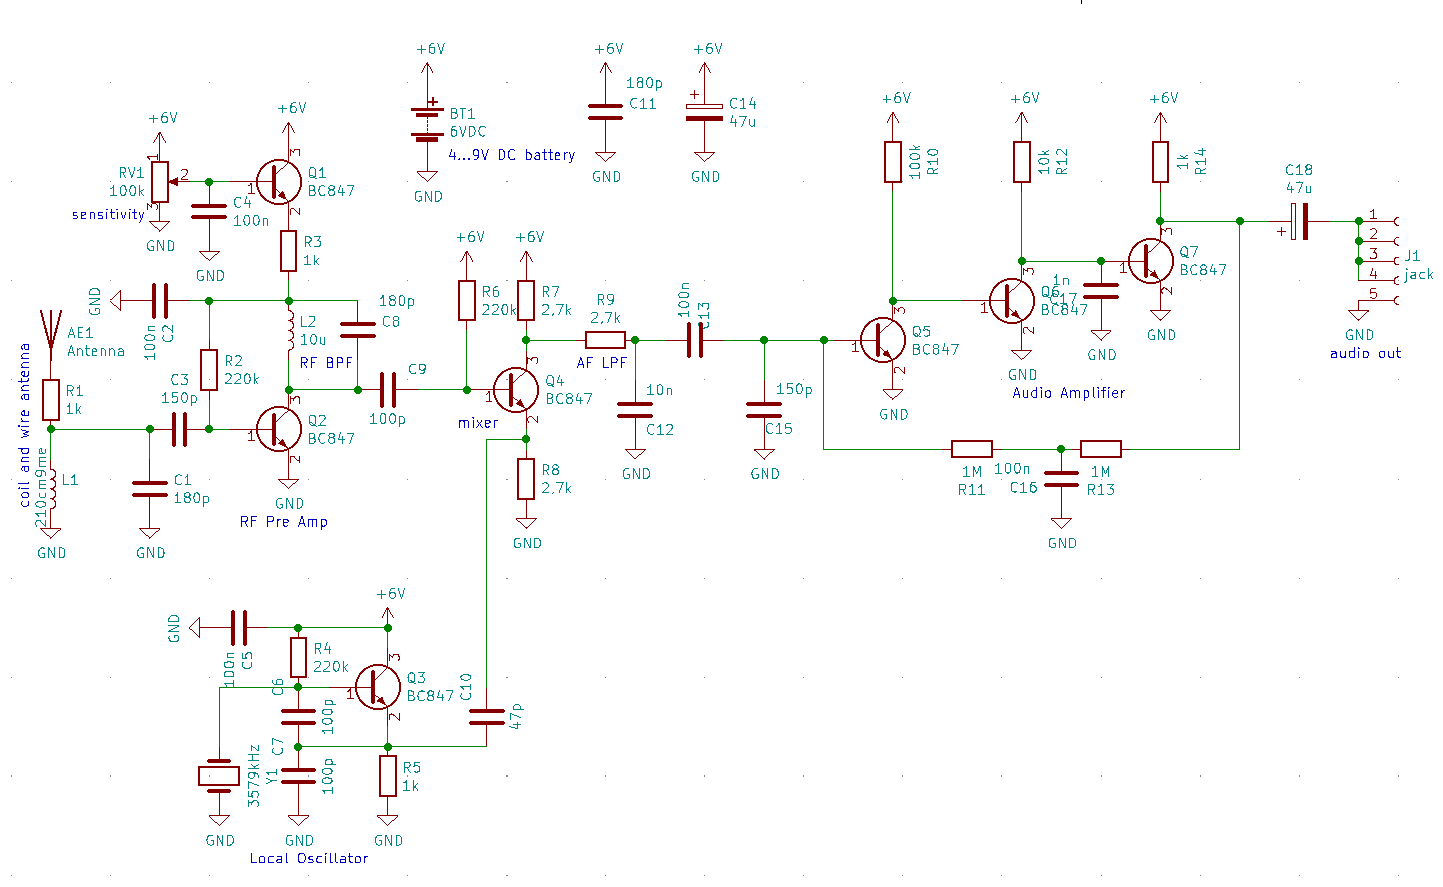
\includegraphics[width=1\textwidth]{../pic/sch.png}\\
\caption{A rókavevő kapcsolási rajza}
\label{fig:rokasch}
\end{figure}

\newpage
\section{Nyomtatott huzalozású lemez}

A NYHL egyoldalas, forrasztásgátló lakkal borított panel - \ref{fig:rokanyhl}. ábra, amely vegyesen furat- és felületszerelt alkatrészeket is tartalmaz.

\begin{figure}[H]
\centering
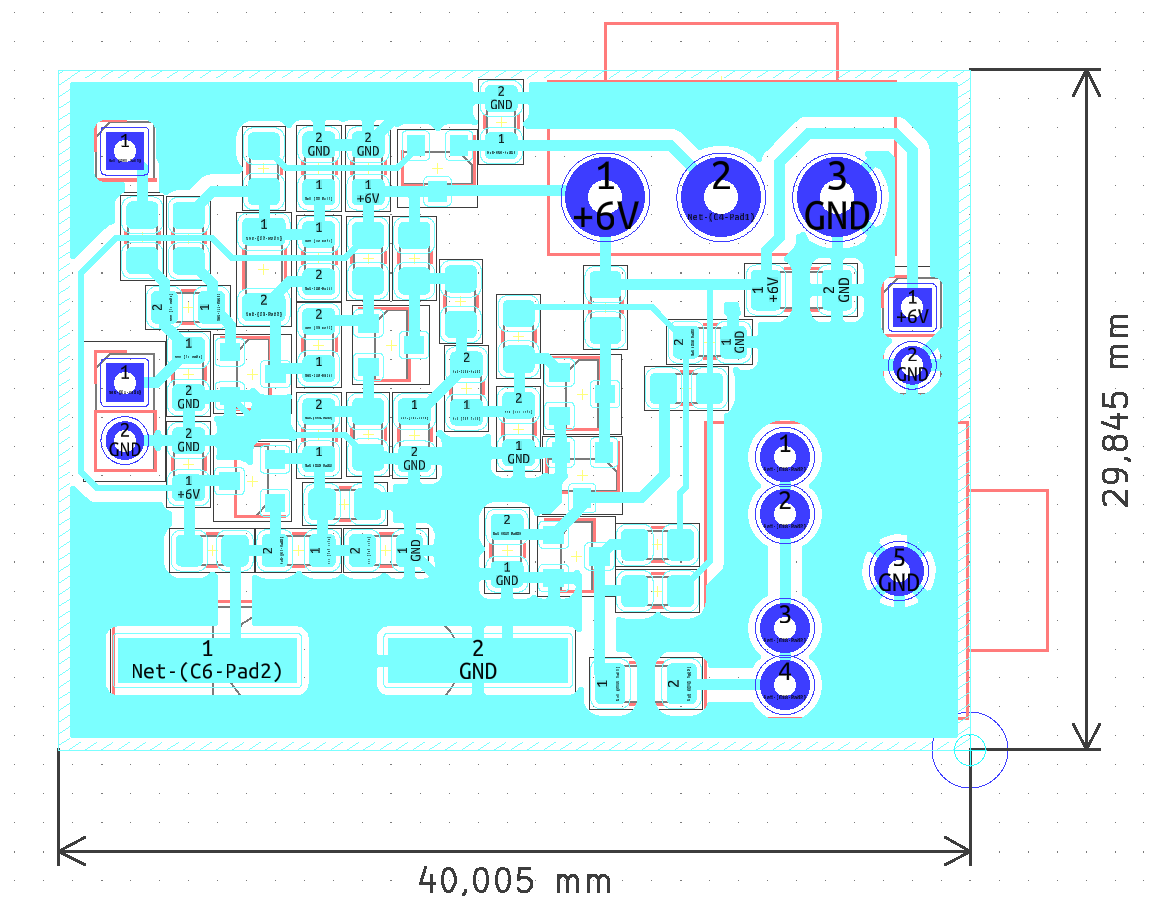
\includegraphics[width=1\textwidth]{../pic/pcb.png}
\caption{HYHL}
\label{fig:rokanyhl}
\end{figure}

\newpage
\section{Alkatrész ültetési rajz}

Az alkatrészek ültetési rajza - a különböző rétegekkel és feliratokkal - \aref{fig:rokault}. ábrán látható.

\begin{figure}[H]
\centering
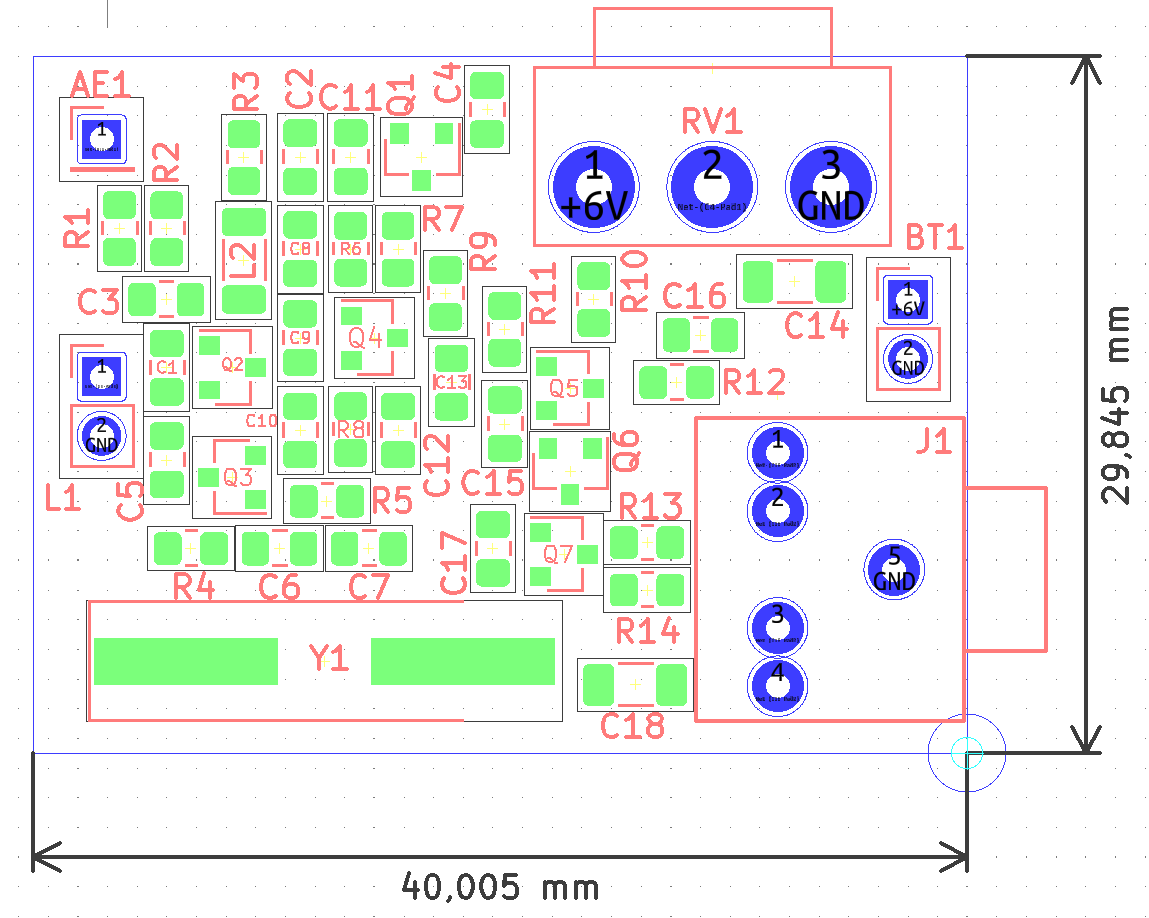
\includegraphics[width=1\textwidth]{../pic/pos.png}
\caption{Az alkatrészek elhelyezése}
\label{fig:rokault}
\end{figure}

Ültetési sorrend:

\begin{enumerate}
\item ellenállások,
\item kondenzátorok,
\item induktivitás (nem az antenna),
\item tranzisztorok,
\item csatlakozók,
\item antenna.
\end{enumerate}

\newpage
\section{Élesztés}

A rendelkezésre álló szárazelemekről indítva a vevő (hibátlan forrasztás esetén) azonnal működőképes.

\section{Mérési feladatok}

Oszcilloszkóp segítségével mérje meg a következőket:

\begin{enumerate}
\item Munkaponti DC feszültségek minden félvezető minden lábán a GND-hez (negatív telepcsatlakozási pont) képest.
\item Vevő helyi oszcillátor jelalak, $V_{pp}$, frekvencia az oszcillátor tranzisztor emitterén.
\item Vevő hangfrekis kimenet a jack csatlakozó meleg pontján a potméter min, közép és max. állásában: jelalak, $V_{pp}$ és frekvencia. - ekkor adott távolságból egy teszt adó fog üzemelni.
\end{enumerate}